\begin{frame}{Vertices and tracks}
\begin{columns}[c]
    \column{.5\textwidth}
    \begin{block}{Vertices}
      \begin{itemize}
          \item Events contain $\approx 7$ Primary Vertices (PVs)
          \begin{itemize}
            \item A PV should contain 5+ long tracks
          \end{itemize}
          \item Multiple Secondary Vertices (SVs) per event as well
          \begin{itemize}
            \item A SV should contain 2+ tracks
          \end{itemize}
      \end{itemize}
    \end{block}

    \column{.5\textwidth}
    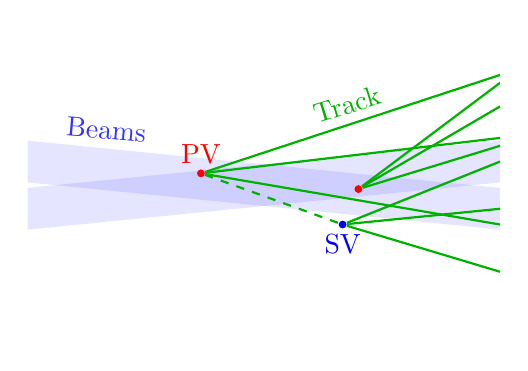
\begin{tikzpicture}
        [beam/.style={line width = 15, opacity=.1, blue, shorten >= -.2cm, shorten <= -.2cm},
        PV/.style={red, circle, fill, inner sep=1pt},
        SV/.style={blue, circle, fill, inner sep=1pt},
        track/.style={green!70!black, thick}]

        \clip [use as bounding box] (-3,-2) rectangle (3,2);
        \clip (-3,-2) rectangle (3,2);

        \node [blue!80!white, rotate=-5] at (-2, .7) {Beams};
        \draw [beam] (-3,.3) -- (3,-.3);
        \draw [beam] (-3,-.3) -- (3,.3);

        \node [PV] (A) at (1.2, -.05) {};
        \node [PV] (B) at (-.8, .15) {};
        \node [red, above] at (B) {PV};

        \draw [track] (A) -- (3,1.3);
        \draw [track] (A) -- (3,1);
        \draw [track] (A) -- (3,.5);

        \draw [track] (B) -- (3,1.4) node [midway, above, rotate=17] {Track};
        \draw [track] (B) -- (3,.6);
        \draw [track] (B) -- (3,-.5);
        \draw [track, dashed] (B) -- (1,-.5);

        \node [SV] (C) at (1,-.5) {};
        \node [blue, below] at (C) {SV};
        \draw [track] (C) -- (3, -.3);
        \draw [track] (C) -- (3, .3);
        \draw [track] (C) -- (3, -1.1);
    \end{tikzpicture}
  \end{columns}

  \begin{block}{}
  \begin{itemize}
      \item We are developing a way to find PVs and SVs using hit triplets
      \item This will enable an iterative tracking algorithm
  \end{itemize}
  \end{block}
\end{frame}
